\newpage
\section{Auswertung}

\subsection{Untersuchung der Filterkurve des Selektivverstärkers}
Die zur Untersuchung der Filterkurve des Selektivverstärkers aufgenommenen Messwerte sind in Tabelle \ref{tab:selektiv} zu finden. Die Filterkurve selbst ist in Abbildung \ref{fig:selektiv} zu sehen.
Es ist zu erkennen, dass das Maximum der Kurve $0{,}47\,\symup{V}$ bei einer Frequenz von $35{,}2\cdot10^{3}\,\symup{Hz}$ beträgt. Bei dieser Frequenz wird die Spannung also ungefiltert durchgelassen.

\begin{table}[htbp]
\centering
\caption{Messwerte zur Untersuchung des Selektivverstärkers. }
\label{tab:selektiv}
\begin{tabular}{S[table-auto-round, table-format=1.3] S[table-auto-round, table-format=1.3] S S}
\toprule
{$U_{\text{A}}/ \, \symup{V}$} & {$\nu/10^{3}\, \symup{Hz}$} & {$U_{\text{A}}/ \, \symup{V}$} & {$\nu/10^{3}\, \symup{Hz}$} \\
\midrule
0.008 & 25.6 & 0.385 & 35.3 \\
0.01 & 27.2 & 0.29 & 35.4 \\
0.014 & 29.1 & 0.23 & 35.5 \\
0.0175 & 30.1 & 0.18 & 35.6 \\
0.021 & 31.1 & 0.17 & 35.7 \\
0.024 & 31.4 & 0.14 & 35.8 \\
0.027 & 31.8 & 0.12 & 35.9 \\
0.03 & 32.1 & 0.11 & 36 \\
0.034 & 32.5 & 0.1 & 36.1 \\
0.043 & 33.0 & 0.098 & 36.2\\
0.0475 & 33.2 & 0.088 & 36.3 \\
0.05 & 33.3 & 0.084 & 36.4 \\
0.054 & 33.4 & 0.075 & 36.5 \\
0.057 & 33.5 & 0.07 & 36.6 \\
0.06 & 33.6 & 0.065 & 36.7 \\
0.066 & 33.7 & 0.06 & 36.8 \\
0.072 & 33.8 & 0.057 & 36.9 \\
0.078 & 33.9 & 0.054 & 37 \\
0.081 & 34 & 0.053 & 37.1 \\
0.086 & 34.1 & 0.048 & 37.3 \\
0.096 & 34.2 & 0.043 & 37.5 \\
0.1 & 34.3 & 0.039 & 37.8 \\
0.12 & 34.4 & 0.036 & 38 \\
0.135 & 34.5 & 0.033 & 38.3 \\
0.16 & 34.6 & 0.0275 & 38.9 \\
0.19 & 34.7 & 0.025 & 39.3 \\
0.23 & 34.8 & 0.024 & 39.5 \\
0.30 & 34.9 & 0.022 & 40 \\
0.47 & 35.2 & & \\
\bottomrule
\end{tabular}
\end{table}

\begin{figure}[h!tbp]
	\centering
	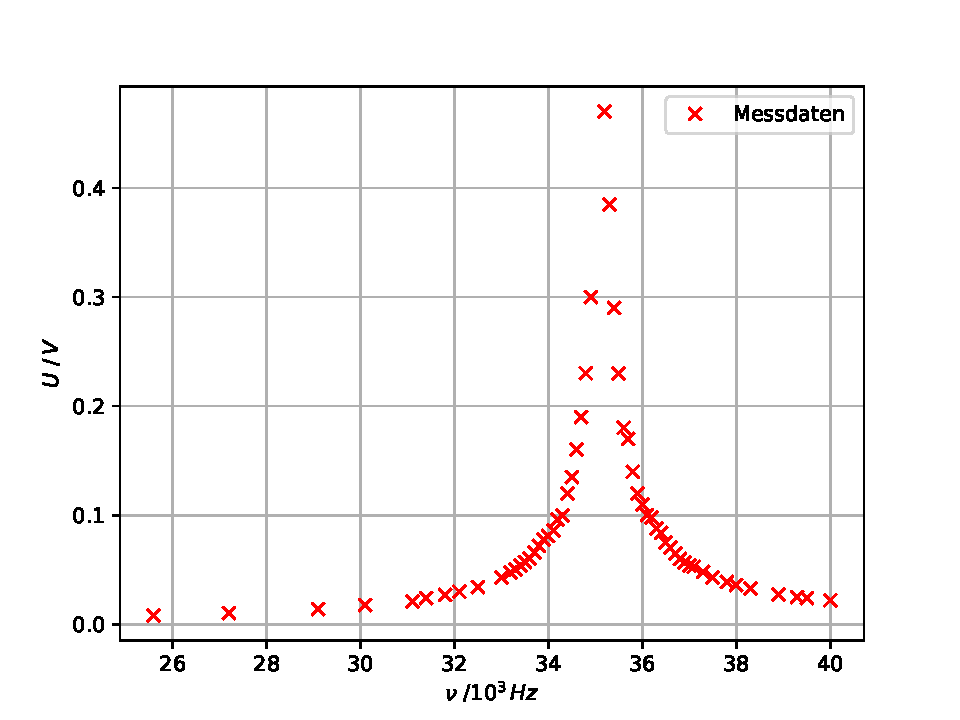
\includegraphics[width=0.9\linewidth]{selektiv.pdf}
	\caption{Filterkurve des Selektivverstärkers.}
	\label{fig:selektiv}
\end{figure}

\newpage
\subsection{Theoretische Bestimmung der Suszeptibilität}
Zunächst wird der theoretische Wert $\chi_{\text{T}}$ der Suszeptibilität der einzelnen Proben bestimmt. Hierzu werden die Gesamtdrehimpulse $J$, die Landé-Faktoren $g_{\text{J}}$, sowie die Anzahl $N$ der magnetischen Momente benötigt.

Die Quantenzahlen - also der Spin $S$, der Bahndrehimpuls $L$ und der Gesamtdrehimpuls $J$ - können mit den Hundschen Regeln bestimmt werden. Aus diesen wiederum werden über Formel \ref{eqn:lande} die Landé-Faktoren berechnet.
Es ergibt sich für die jeweiligen Proben:

\begin{table}[htbp]
\centering
\caption{Werte zur theoretischen Bestimmung der Suszeptibilität.}
\label{tab:some_data}
\begin{tabular}{S[table-auto-round, table-format=1] S[table-auto-round, table-format=1.2] S S}
\toprule
 & {$Gd_2O_3 $} & {$Dy_2O_3$} & {$Nd_2O_3$} \\
\midrule
S & 3.5 & 2.5 & 1.5 \\
L & 0   & 5   & 6  \\
J & 3.5 & 7.5 & 7.5  \\
$g_{\text{J}}$ & 2 & 1.33 & 0.73 \\
\bottomrule
\end{tabular}
\end{table}

Die Berechnung der Anzahl $N$ der magnetischen Momente geschieht über folgenden Ansatz, wobei $m$ die Masse ist, $\rho$ die Dichte des Stoffes, $V$ das Volumen, $n$ die Stoffmenge und $M$ die molare Masse:

\begin{equation}
\begin{aligned}
m &= \rho \cdot V = M \cdot n\\
\iff \frac{n}{V} &= \frac{\rho}{M} \\
\iff N &= \frac{\rho}{M} \\
\end{aligned}
\end{equation}

Die Dichten werden aus der Versuchseinleitung \cite[14]{anleitung606} entnommen, die molaren Massen \cite{molaremasse} werden mit $1\,u = 1{,}661\cdot10^{-27}\,\symup{kg}$ umgerechnet:

\begin{table}[htbp]
\centering
\caption{Werte zur theoretischen Bestimmung der Suszeptibilität.}
\label{tab:some_data}
\begin{tabular}{S[table-figures-exponent=2] S[table-auto-round, table-format=1.2] S S}
\toprule
 & {$Gd_2O_3 $} & {$Dy_2O_3$} & {$Nd_2O_3$} \\
\midrule
M/e-25\,$\symup{kg}$& 6.02 & 6.19 & 5.59 \\
N/e28\,$\symup{\frac{1}{m^3}}$ & 1.23   & 1.26  & 1.29  \\
\bottomrule
\end{tabular}
\end{table}

Nach Einsetzen aller Werte in Formel \ref{eq:mariecurie}, wobei für die Konstanten

\begin{equation*}
\begin{aligned}
\mu_0          &= 1{,}256\cdot10^{-6}\,\symup{\frac{N}{A^2}} \\
\mu_{\text{B}} &= 9{,}274\cdot10^{-24}\,\symup{\frac{J}{T}} \\
k              &= 1{,}38 \cdot10^{-23}\,\symup{\frac{J}{K}} \\
\end{aligned}
\end{equation*}

eingesetzt und für die Temperatur $T=294{,}15\,\symup{K}$ angenommen wird, ergeben sich die folgenden theoretischen Werte der Suszeptibilität:

\begin{equation}
\begin{aligned}
\chi_{\text{T,Gd}} &= 0{,}0069 \\
\chi_{\text{T,Dy}} &= 0{,}0126 \\
\chi_{\text{T,Nd}} &= 0{,}0039 \\
\end{aligned}
\end{equation}






\subsection{Experimentelle Bestimmung der Suszeptibilität über die Widerstandsdifferenz}
Zur Bestimmung der Suszeptibilität der Proben über die Widerstandsdifferenzen wird der Querschnitt der Spule $F = 8{,}66\cdot10^{-5}\,\symup{m^2}$, der Querschnitt $Q$ der Probe, 
der Widerstand $R_3 = 998\,\symup{\Omega}$ und die Widerstandsdifferenz $\Delta R$ benötigt.

Zur Berechnung des Querschnitts $Q$ werden die Masse $m$, die Länge $l$ und die Dichte $\rho$  benötigt. Diese sind für die einzelnen Proben gegeben durch:

\begin{table}[htbp]
\centering
\caption{Werte zur Berechnung des Querschnitts Q.}
\label{tab:some_data}
\begin{tabular}{S[table-figures-exponent=1] S[table-auto-round, table-format=4.2] S S}
\toprule
 & {$Gd_2O_3 $} & {$Dy_2O_3$} & {$Nd_2O_3$} \\
\midrule
$m$/e-3\,$\symup{kg}$& 14.08 & 15.1 & 9 \\
$l$/e-2\,$\symup{m}$ & 17.5  & 17.5  & 17.4  \\
$\rho$/\,$\symup{\frac{kg}{m^3}}$ & 7400 & 7800 & 7240 \\
\bottomrule
\end{tabular}
\end{table}
$Q$ kann nun über die Formel

\begin{equation*}
Q = \frac{m}{L\cdot\rho}
\end{equation*}
berechnet werden. Die Querschnitte der Proben betragen damit:

\begin{equation*}
\begin{aligned}
Q_{\text{Gd}} &= 10{,}87\cdot10^{-6}\,\symup{m^2} \\
Q_{\text{Dy}} &= 11{,}06\cdot10^{-6}\,\symup{m^2} \\
Q_{\text{Gd}} &= 7{,}17\cdot10^{-6}\,\symup{m^2} \\
\end{aligned}
\end{equation*}

Da für jede der Proben drei Messungen durchzuführen sind, werden die Messwerte der Widerstände zunächst gemittelt und es wird anschließend eine Fehlerrechnung durchgeführt.
Allgemein ergibt sich der Mittelwert durch

\begin{equation}
\bar{R} = \frac{1}{N} \sum_{i=1}^N R_i
\end{equation}
und der Fehler des Mittelwerts durch

\begin{equation}
\Delta \bar{R} = \frac{1}{\sqrt{N}} \sqrt{\frac{1}{N-1}\sum_{i=1}^N (R_i - \bar{R})^2}.
\end{equation}
Dies liefert die folgenden Werte:

\begin{table}[h!tbp]
\centering
\caption{Werte zur Bestimmung der Suszeptibilität von $Gd_2O_3$. }
\label{tab:some_data}
\begin{tabular}{S[table-format=4] S S[table-auto-round, table-format=3] S[table-auto-round, table-format=3.1] S}
\toprule
{$R_0/ 10^{-3}\, \symup{\Omega}$} & {$R_{\text{m}}/ 10^{-3}\, \symup{\Omega}$} & {$\Delta R/ 10^{-3}\, \symup{\Omega}$} & {$\bar{R}/ 10^{-3}\, \symup{\Omega}$} & {$\Delta \bar{R}/ 10^{-3}\, \symup{\Omega}$}\\
\midrule
3080 & 2320 & 760 & 885 & 150.7 \\
3300 & 2115 & 1185 \\
2950 & 2240 & 710 \\
\bottomrule
\end{tabular}
\end{table}


\begin{table}[h!tbp]
\centering
\caption{Werte zur Bestimmung der Suszeptibilität von $Dy_2O_3$. }
\label{tab:some_data}
\begin{tabular}{S[table-format=4] S S[table-auto-round, table-format=3] S[table-auto-round, table-format=3.1] S}
\toprule
{$R_0/ 10^{-3}\, \symup{\Omega}$} & {$R_{\text{m}}/ 10^{-3}\, \symup{\Omega}$} & {$\Delta R/ 10^{-3}\, \symup{\Omega}$} & {$\bar{R}/ 10^{-3}\, \symup{\Omega}$} & {$\Delta \bar{R}/ 10^{-3}\, \symup{\Omega}$} \\
\midrule
3235 & 1490 & 1745 & 1685 & 32.15\\
3040 & 1405 & 1635 \\
3185 & 1510 & 1675 \\
\bottomrule
\end{tabular}
\end{table}


\begin{table}[h!tbp]
\centering
\caption{Werte zur Bestimmung der Suszeptibilität von $Nd_2O_3$.}
\label{tab:some_data}
\begin{tabular}{S[table-format=4] S S[table-auto-round, table-format=3] S[table-auto-round, table-format=3.1] S}
\toprule
{$R_0/ 10^{-3}\, \symup{\Omega}$} & {$R_{\text{m}}/ 10^{-3}\, \symup{\Omega}$} & {$\Delta R/ 10^{-3}\, \symup{\Omega}$} & {$\bar{R}/ 10^{-3}\, \symup{\Omega}$} & {$\Delta \bar{R}/ 10^{-3}\, \symup{\Omega}$}\\
\midrule
3060 & 2755 & 305 & 266.67 & 46.04 \\
3125 & 2805 & 320 \\
3120 & 2945 & 175 \\
\bottomrule
\end{tabular}
\end{table}
Zuletzt werden $\bar{R}$ und $\Delta\bar{R}$ der jeweiligen Proben, sowie die Querschnitte $Q$ und $F$ in die Formel \ref{eqn:chiwiderstand} eingesetzt. Hieraus ergeben sich experimentellen Werte der Suszeptibilität
der verschiedenen Materialien:

\begin{equation}
\begin{aligned}
\chi_{\text{R,Gd}} &= 0{,}0014 \pm 0{,}002 \\
\chi_{\text{R,Dy}} &= 0{,}0269 \pm 0{,}0005 \\
\chi_{\text{R,Nd}} &= 0{,}0043 \pm 0{,}0007 \\
\end{aligned}
\end{equation}
